%!TEX root = ../template.tex
%%%%%%%%%%%%%%%%%%%%%%%%%%%%%%%%%%%%%%%%%%%%%%%%%%%%%%%%%%%%%%%%%%%%
%% chapter2.tex
%% NOVA thesis document file
%%
%% Chapter with the template manual
%%%%%%%%%%%%%%%%%%%%%%%%%%%%%%%%%%%%%%%%%%%%%%%%%%%%%%%%%%%%%%%%%%%%

\typeout{NT FILE chapter2.tex}%

\chapter{Company and LEAP-1A Overview}
\label{cha:enquadramento}

%\glsresetall

\section{TAP M\&E}
\label{sec:empresa}

\gls{TAP} was founded in 1945, during the end of World War II, a period marked by significant development in the aviation industry. 

\gls{TAP} \gls{ME} is responsible for performing maintenance and engineering support services to \gls{TAP}'s airline fleet and third-party customers. Services such as Aircraft Maintenance, Engine Repair and Overhaul and Components Repair and Overhaul.

To maintain \gls{TAP} Air Portugal's reputation as one of the most reliable airlines in the world, \gls{TAP} \gls{ME} embraces the concept of \textit{Care2Quality}. This philosophy is founded on three key pillars: \textbf{Safety}, \textbf{Quality}, and \textbf{Relationships}. It is integrated across all \gls{TAP} \gls{ME} products and services, which are organized into five main departments: \textit{Care2Airframe}, \textit{Care2Engines}, \textit{Care2Components}, \textit{Care2Engineering}, and \textit{Care2Technical Labs}.

\gls{TAP} \gls{ME} offers extensive \gls{MRO} services for a variety of aircraft systems and engine models. For \gls{CFMI} engines, including the CFM56 series and \gls{LEAP}-1A, it provides light and heavy maintenance, engine testing, troubleshooting, redelivery checks, technical consulting, and engine trend monitoring.

Currently in its fleet \gls{TAP} has the following aircraft:

\begin{table}[h!]
    \caption{\gls{TAP} Air Fleet Composition \cite{aviacaocomercial}}
    \label{tab:tap_aircraft}
    \centering
    \begin{tabular}{ccc}
    \hline
    \textbf{Aircraft} & \textbf{Active N\textsuperscript{o}} & \textbf{Age} \\ \hline
    Airbus A319ceo                 & 3          & 23         \\ 
    Airbus A320ceo                 & 15         & 19         \\ 
    Airbus A320neo              & 15         & 3          \\ 
    Airbus A321ceo                 & 3          & 22         \\ 
    Airbus A321neo              & 12         & 4          \\ 
    Airbus A321LRneo            & 11         & 3          \\ 
    Airbus A330ceo             & 3          & 16         \\ 
    Airbus A330neo          & 19         & 5          \\ \hline
    \end{tabular}
    \end{table}

\section{LEAP Engine}
\label{sec:motor_leap}

\gls{LEAP} engine family, developed and produced by CFM International—a joint venture between Safran Aircraft Engines and GE Aerospace—continues the legacy of the CFM56 as a best-seller in commercial aviation. Introduced in 2016, the LEAP powers the Airbus A320neo, Boeing 737 MAX, and COMAC C919, delivering a 15\% improvement in fuel efficiency, along with reduced noise and emissions, while maintaining industry-leading reliability and cost-effectiveness. This advanced engine reflects the enduring success of the partnership between Safran and GE, which has been extended until 2050.

The \gls{LEAP}, like most modern commercial aircraft engines, is a turbofan engine.

\subsection{Turbofan}
\label{subsec:turbofan}

The Turbofan engine applies the same principle as the turbojet and all jet engines, Newton's third law: "For every action, there is an equal and opposite reaction".
In this case, the first object is the engine itself and the second is the atmospheric air that is forced to accelerate as it passes through the engine causing the airplane to move forward. 

To understand how the turbofan engine works, it is a good approach to analyze the turbojet working cycle and how it is processed first.  
As shown in Figure~\ref{fig:turbojet} the working cycle of a TurboJet has 4 main stages: Air intake, Compression, Combustion and Exhaust.
At intake, the air is at atmospheric pressure, but as it passes through the compressors, it is compressed to optimal pressure and temperature conditions for combustion. Upon entering the combustion chamber, fuel nozzles mix the fuel and air, creating a homogeneous mixture that minimizes the peak temperature during combustion.
During the combustion process, this mixture burns at constant pressure, increasing the air's volume while causing a decrease in pressure. The gases resulting from combustion expand through the turbine and jet pipe back to atmosphere providing the force needed to propel the airplane forward. During this part of the cycle, some of the energy in the expanding gases is turned into mechanical power by the turbine. 

\begin{figure}[H]
    \centering
    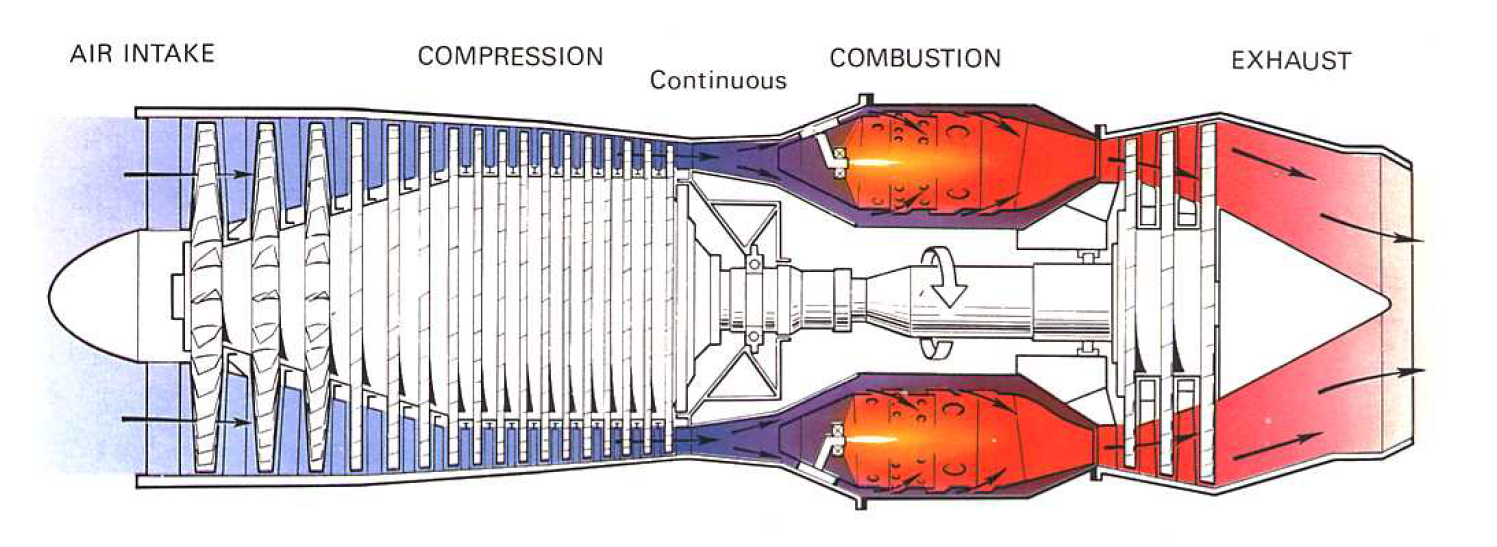
\includegraphics[width=1\textwidth]{TurboJet}
    \caption{TurboJet Engine Work Cycle stages.\cite{RollsRoyce}}
    \label{fig:turbojet}
\end{figure}

Analysing the Turbofan work cycle requires a more complex approach since the air that goes through the combustor is now only responsible for 20\% of the thrust power.

At the start, the engine's high-pressure shaft receives mechanical power with the assistance of a system called the Air Turbine Starter. This rotation drives the compressor blades, drawing air through the engine and initiating the compression process. The airflow through the engine also causes the fan to start moving. Once the engine reaches 20\% of its maximum RPM, sufficient compression is generated to initiate combustion. With everything in motion, the engine enters a cycle similar to the turbojet working cycle. The gases produced from combustion expand through the \gls{HP} and \gls{LP} turbines, delivering mechanical power to the \gls{HP} and \gls{LP} shafts. These shafts, in turn, transmit rotational energy to the \gls{HP} and \gls{LP} compressors as well as the front fan.
As the fan rotates at high speed, it separates the incoming air into two distinct streams, forming the bypass ratio. Commercial aircraft engines, such as the LEAP-1A, are high-bypass ratio engines. In these engines, one stream of air enters the engine core, powering the turbojet-like working cycle. The remaining air, approximately 80\% of the total intake, is channeled around the engine core. This bypassed air is directed into a narrow passage known as the fan duct, where its speed increases significantly. This accelerated airflow generates the majority of the thrust required to lift the aircraft.  

In summary, the main differences between turbofan and turbojet engines lie in their airflow management and structural design. A key distinction is the large fan at the front of the turbofan, which directs a significant portion of the air around the engine core, defining the bypass ratio, which is the ratio of the amount of air bypassing the core to the amount of air passing through it, as illustrated in Figure~\ref{fig:turbofan}.
Wheight wise, for the same power output, given the fact that all the high pressure rotating assemblies diameter can be reduced, the turbofan engines are lighter, improving the power-wheight ratio of the engine. A low bypass ratio engine has a wheight reduction of 20 percent compared to a pure jet engine for the same air mass flow.\cite{RollsRoyce}
Another significant advancement in turbofan engines is the introduction of the multi-spool or multi-shaft system, although this technology can also be applied to pure jet engines. The presence of both \gls{LP} and \gls{HP} turbines and compressors requires each assembly to rotate at different speeds, since just a percentage of the air that flows through the \gls{LP} Compressor goes into the \gls{HP} one (the majority of the air forms the bypass flow). This is essential for achieving higher efficiency, as each component operates at its optimal rotational velocity. 
Most commercial aircraft engines are high-bypass engines, and the typical configuration for these engines is a two-shaft system. As illustrated in Figure~\ref{fig:turbofan} the \gls{LP} compressor is powered by a shaft coming from the \gls{LP} turbine, and the same applies to the \gls{HP} spool.

\begin{figure}[H]
    \centering
    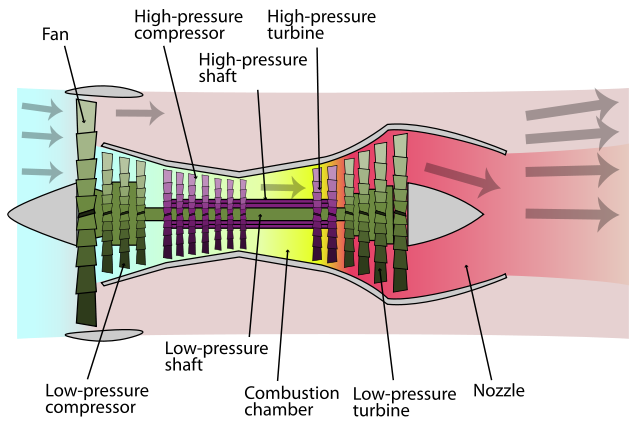
\includegraphics[width=0.8\textwidth]{Turbofan}
    \caption{Turbofan Engine. \cite{Aainsqatsi2008}}
    \label{fig:turbofan}
\end{figure}

\subsection{LEAP Family}
\label{subsec:leapfamily}
As mentioned at the beginning of this chapter, the LEAP engine powers a variety of aircraft, with its characteristics varying depending on the application. 
Therefore, we can categorize the \gls{LEAP} engine family based on application and thrust power.

\begin{figure}[H]
    \centering
    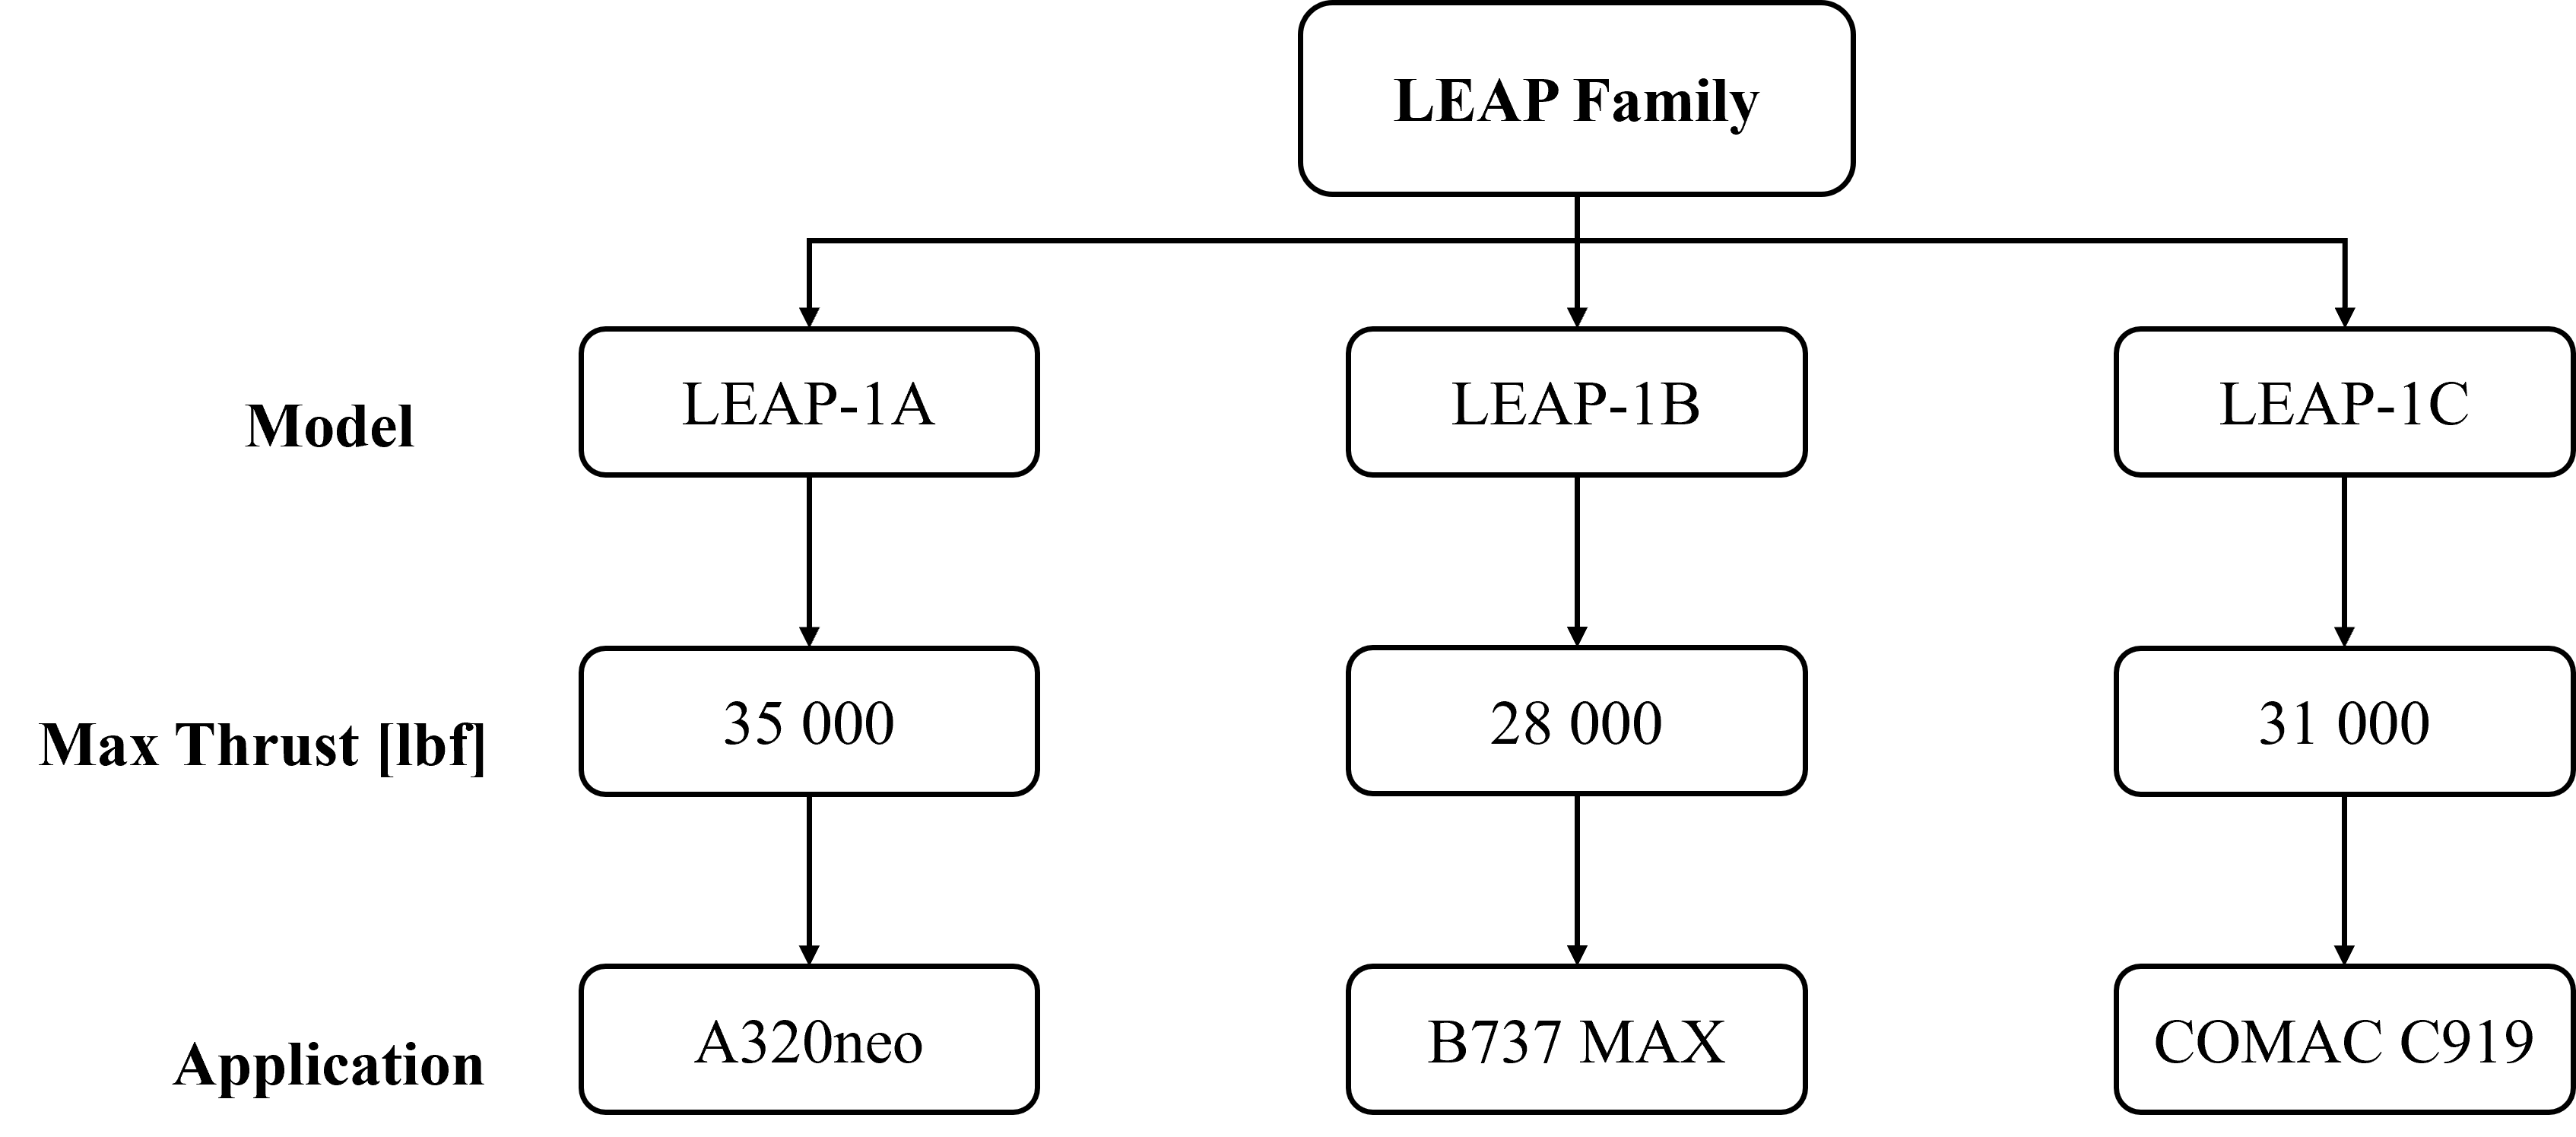
\includegraphics[width=0.8\textwidth]{leapfamily}
    \caption{\gls{LEAP} Family.\cite{brochureleap}}
    \label{fig:leapfamily}
\end{figure}

Each model also has variations based on its thrust. For instance, the \gls{LEAP}-1A can be further subcategorized into \gls{LEAP}-1A23, \gls{LEAP}-1A24, \gls{LEAP}-1A26, \gls{LEAP}-1A30, \gls{LEAP}-1A32, \gls{LEAP}-1A33, and \gls{LEAP}-1A35. 
Considering that in '\gls{LEAP}-1A24', the '24' indicates the engine's thrust capacity of 24 klbf.

Currently, in the \gls{TAP} Air Fleet Composition, the LEAP-1A26 and LEAP-1A32 engines are used respectively in the Airbus A320neo and A321neo.


\subsection{LEAP-1A}
\label{subsec:leap1a}

The \gls{LEAP}-1A, represented in Figure~\ref{fig:leap1a}, is a high-bypass turbofan engine designed to power the next-generation Airbus A320neo. This section presents some of its key features, along with its main modules and innovations in comparison to its predecessor, the CFM56. Most of this information is derived from the engine’s brochure and training manual.

\begin{figure}[H]
    \centering
    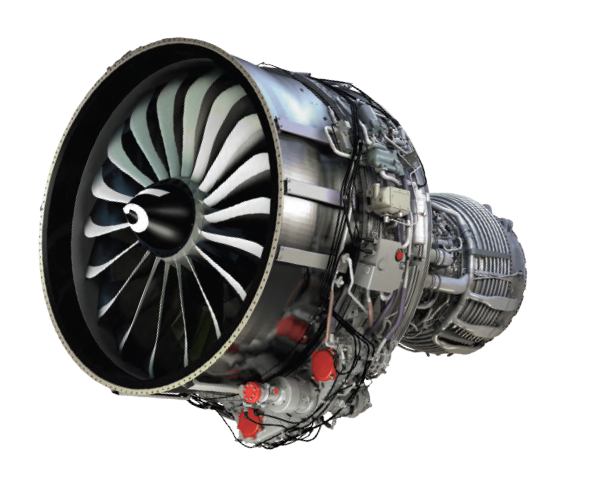
\includegraphics[width=0.7\textwidth]{leap1a}
    \caption{\gls{LEAP}-1A.\cite{brochureleap}}
    \label{fig:leap1a}
\end{figure}

This powerplant is presented with the following characteristics in Table~\ref{tab:leapcha}.
%\cite{mtuleap1a1b}
\begin{table}[ht]
    \caption{Characteristics of the \gls{LEAP}-1A engine.\cite{MTU_LEAP}}
    \label{tab:leapcha}
    \centering
    \begin{tabular}{lc}
    \hline
    \textbf{Characteristic} & \textbf{Value} \\ \hline
    Takeoff thrust                      & Up to 35,000 lbf   \\
    Bypass ratio                        & 11:1                \\
    Overall pressure ratio              & 40:1                \\
    Fan diameter                        & 1.98 m (78 in)      \\
    Compressor stages (fan/booster/HPC) & 1 + 3 + 10          \\
    Turbine stages (HP/LP)              & 2 + 7               \\
    Weight                              & 3007 kg             \\
    Length                              & 3.35 m (11 ft)      \\
    Width                               & 2.53 m (8.3 ft)     \\
    Height                              & 2.38 m (7.8 ft)     \\ \hline
    \end{tabular}
\end{table}



Design and function wise \gls{LEAP}-1A present in its composition 4 Major modules. As represented in Figure~\ref{fig:modules}, Fan and Booster, Core, \gls{LP} Turbine and Accessory Drive Major Modules.

\begin{figure}[H]
    \centering
    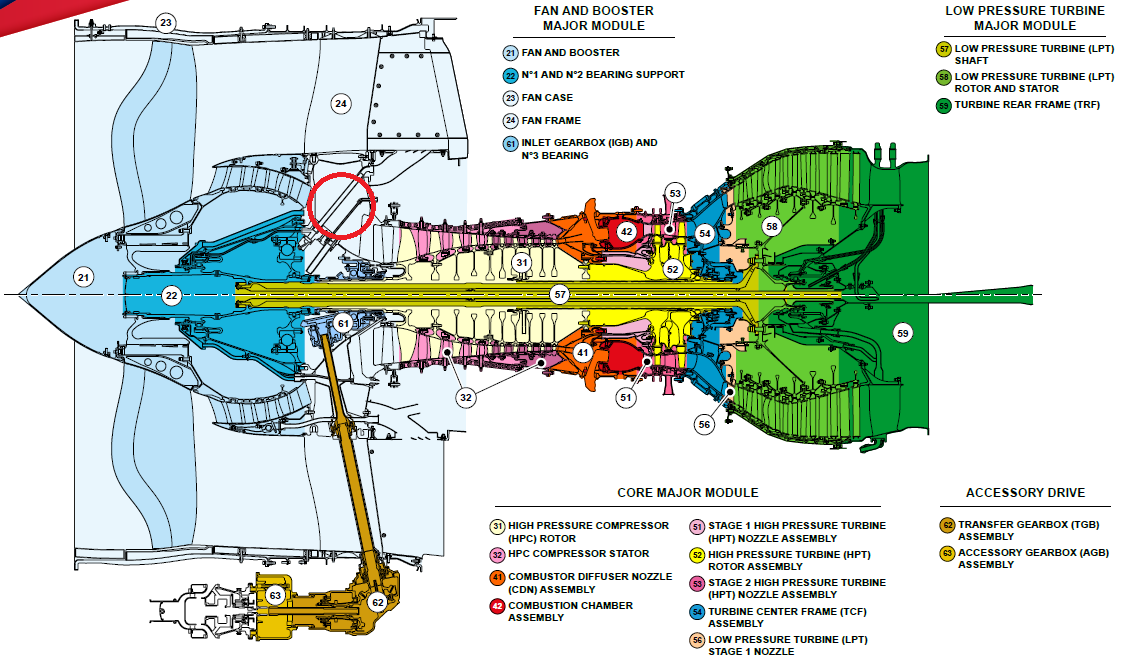
\includegraphics[width=0.8\textwidth]{modulos}
    \caption{\gls{LEAP}-1A Major Modules.\cite{Leeham_HighTurbine}}
    \label{fig:modules}
\end{figure}

    %\cite{fehrm2024bjorns}

\subsubsection{Fan and Booster Major Module}
\label{subsubsec:fan_booster}

As shown in Figure~\ref{fig:modules}, the Fan and Booster Major Module consists of the Fan and Booster itself, two bearing supports, the fan case, the fan frame, the inlet gearbox, and the number 3 bearing.

The Fan and Booster assembly represents the integration of the front fan and the \gls{LP} Compressor.
    
The fan itself is composed of a single assembly that includes one front spinner, 18 fan blades, a flow splitter, and a platform front shroud.
    
The \gls{LPC} consists of three stages: the first stage has 62 blades, the second stage has 75 blades, and the third stage has 72 blades.
    
One of the major technological breakthroughs in the new LEAP-1A engine is the production of its fan blades. These blades are manufactured using additive manufacturing with 3D-woven \gls{RTM} carbon fiber composites. Compared to the solid titanium blades of the CFM56, this advancement allows for larger blades, as illustrated in Figure~\ref{fig:blade_comparison}, without increasing the engine's weight. According to the company, this material helps reduce engine weight by 500 lbs per unit.

\begin{figure}[H]
    \centering
    \includegraphics[width=0.3\textwidth]{comparaçao}
    \caption{\gls{LEAP}-1A fan blades vs CFM56 fan blades.\cite{ESM}}
    \label{fig:blade_comparison}
\end{figure}

In summary, the purpose of this engine assembly is to impart kinetic energy to the incoming airflow, separate the primary and secondary airflow, and expel the hot air generated by the engine.

\subsubsection{Core}
\label{subsubsec:core}

Next is the Core Major Module, which is responsible for generating thrust by producing power through highly compressed air.

This \gls{MM} comprises the assembly of the \gls{HPC}, combustion chamber, and \gls{HPT}. Additionally, it is divided into nine sub-modules.

The \gls{HPC} consists of the HPC rotor and stator, while the \gls{HPT} includes the HPT rotor along with the stage 1 and stage 2 nozzle assemblies. The Core Major Module also incorporates the Turbine Center Frame and the \gls{LPT} Stage 1 Nozzle.

To achieve optimal performance, the \gls{HPC} features 10 stages, as shown in Table~\ref{tab:bladeshpc}. Each stage consists of one rotor and one stator. The first five stages of compression are achieved through blisks, while the remaining five stages use compressor blades with circumferential assembly.
This mini module has the purpose of increasing the pressure of the booster discharge air for combustion.

\begin{table}[ht]
    \caption{Number of blades per stage on HPC \cite{ESM}}
    \label{tab:bladeshpc}
    \centering
    \begin{tabular}{ccccccccccc}
    \toprule
    \textbf{Stage} & 1 & 2 & 3 & 4 & 5 & 6 & 7 & 8 & 9 & 10 \\ \hline
    \textbf{Number of blades} & - & - & - & - & - & 62+2+2 & 57+2+2 & 63+2+2 & 60+2+2 & 64+2+2 \\ \bottomrule
    \end{tabular}
\end{table}
   

It is important to note that the HPC rotor is coupled with the HPT, as shown in Figure~\ref{fig:shafts}. This coupling allows the kinetic energy extracted from the HPT to be used for compressing the airflow. Likewise, the same principle applies to the \gls{LPC} and \gls{LPT}.

In Figure~\ref{fig:shafts}, the yellow assembly represents the Low-Pressure rotor, while the orange assembly corresponds to the High-Pressure rotor.
    
As mentioned in \ref{subsec:turbofan}, these rotors rotate at different speeds. The \gls{LP} rotor operates at N1 speed (3 850 RPM), whereas the \gls{HP} rotor rotates at N2 speed (16 645 RPM).  

\begin{figure}[H]
    \centering
    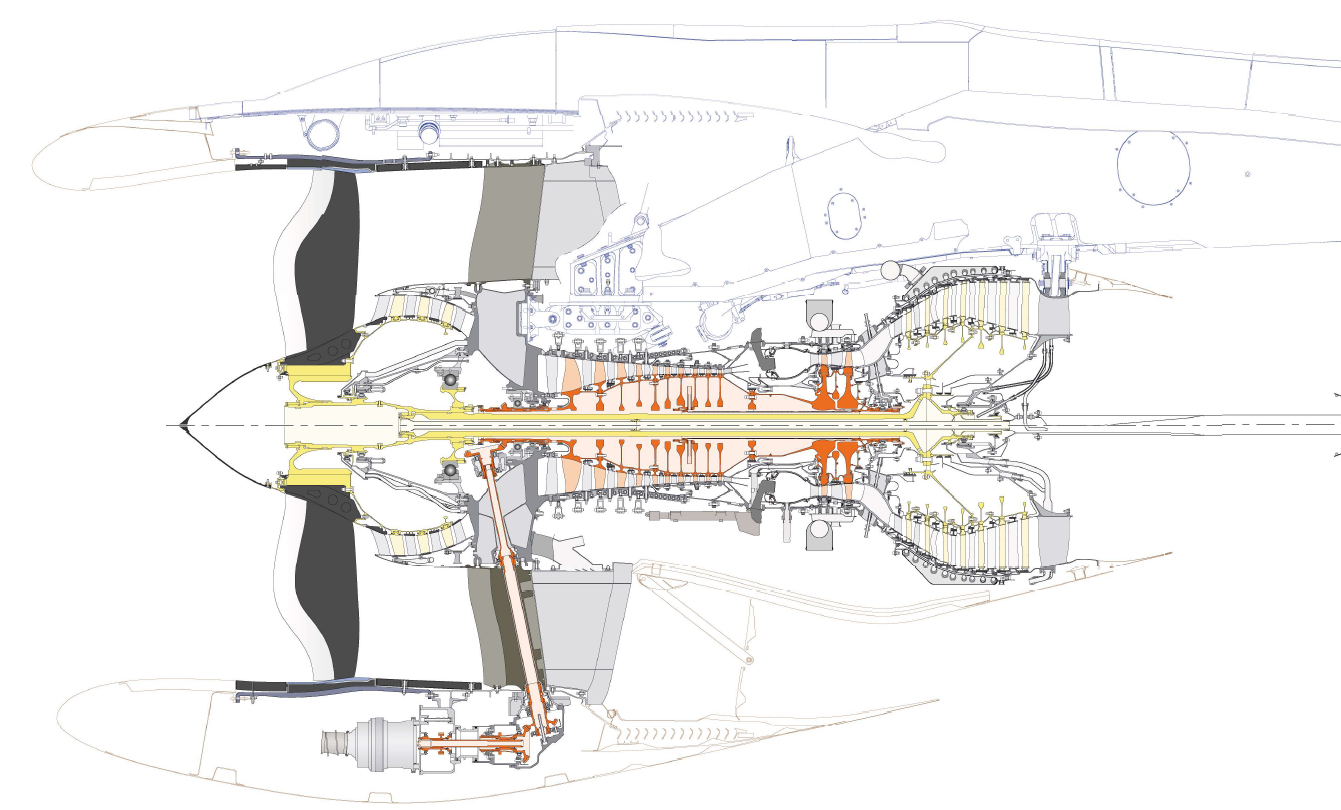
\includegraphics[width=0.8\textwidth]{shafts}
    \caption{High and Low pressure rotors \cite{ESM}}
    \label{fig:shafts}
    \end{figure}
    

    \subsubsection{\gls{LP} Turbine Major Module}
    \label{subsubsec:lp_turbine}

The \gls{LP} Turbine Major Module, represented in Figure~\ref{fig:lpt}, is composed by the \gls{LP} turbine shaft, rotor and stator and the turbine rear frame. 

\begin{figure}[H]
    \centering
    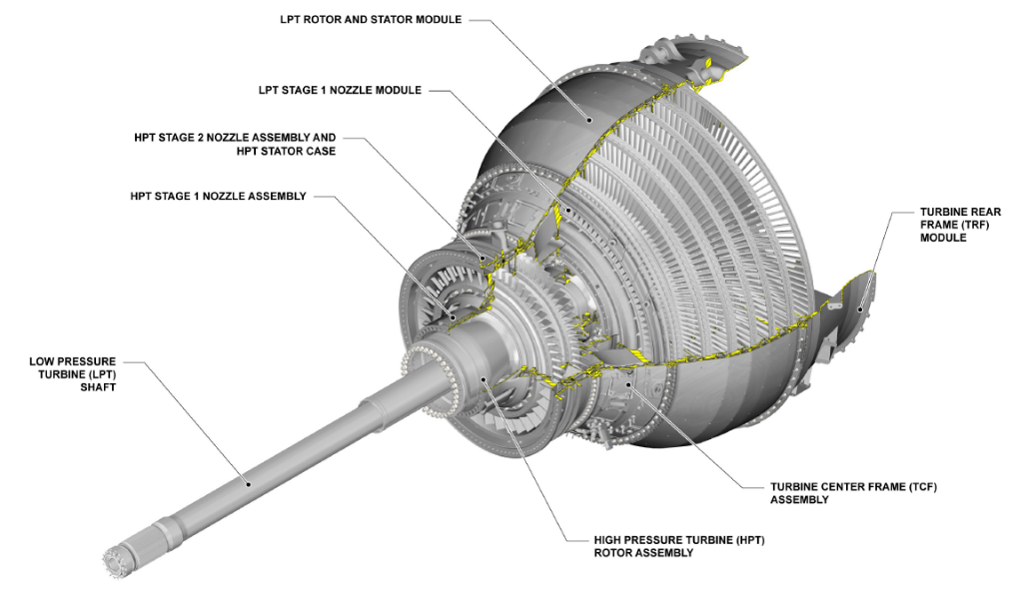
\includegraphics[width=0.8\textwidth]{lptmm}
    \caption{\gls{LPT}. \cite{ESM}}
    \label{fig:lpt}
\end{figure}


Its primary function is to supply mechanical power to the \gls{LP} Compressor by converting the termal energy from the hot gases released from the combustion chambers into kinetic energy while simultaneously decompressing it.

It is worth noting that while both turbines and compressors present similar designs and compositions, their functions are fundamentally opposite.

As previously mentioned, compressors consume energy and transfer it to the air, compressing it while increasing its velocity, whereas turbines absorb energy from the expansion of the combustion gases and convert it into mechanical power.

Both components consist of stages that include one stationary and one rotating element, but their purposes and arrangements differ. As illustrated in Figure~\ref{fig:compressorvsturbine}, in a compressor, a rotor row is followed by a stationary vane row, while in a turbine, a stationary nozzle precedes a rotating rotor row. The stationary vanes in the compressor are responsible for further compressing the air trough diffuion processes, whereas the nozzles in the turbine decompress the airflow and guide it in the most efficient direction, maximizing the kinetic energy absorbed by the turbine blades.

A more detailed explanation of the compressor's operation is provided in the following sections.

\begin{figure}[H]
    \centering
    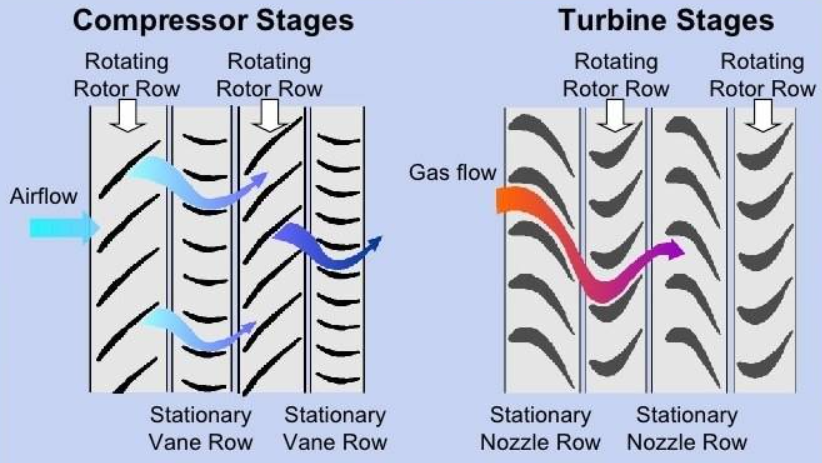
\includegraphics[width=0.6\textwidth]{compressorvsturbine}
    \caption{Axial Compressor vs Turbine flow \cite{trent1}}
    \label{fig:compressorvsturbine}
\end{figure}

    \subsubsection{Accessory Drive}
    \label{subsubsec:accessory_drive}

As shown in Figure~\ref{fig:drives}, the accessory drive delivers torque to the HPC to initiate engine start-up, as described in \ref{subsec:turbofan}, enabling the compression process (red arrow path). During the engine’s operating cycle, it supplies mechanical energy to both the aircraft and engine accessories (orange arrow path).

\begin{figure}[H]
    \centering
    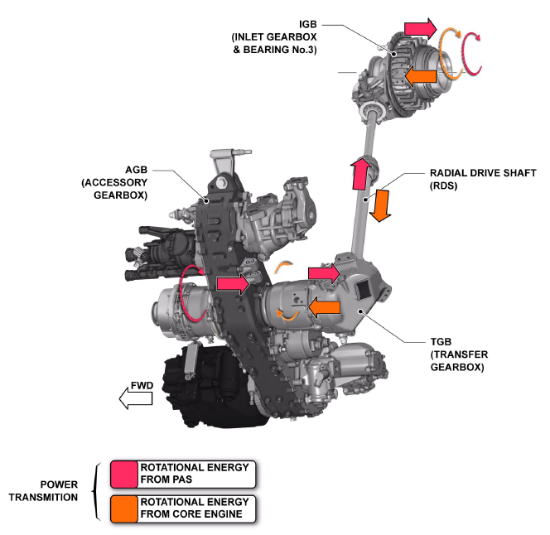
\includegraphics[width=0.5\textwidth]{drives}
    \caption{LEAP-1A Accessory Drives.\cite{ESM}}
    \label{fig:drives}
\end{figure}




































